\hypertarget{othello-frontend-othello.ipynb}{%
\section{Othello Frontend
(othello.ipynb)}\label{othello-frontend-othello.ipynb}}

\label{sec:frontend}

\begin{lstlisting}[language=Python]
%%HTML
<style>
.container { width:100% }
</style>
\end{lstlisting}

Dieses Notebook dient als Benutzerschnittstelle, über die ein
menschlicher Spieler gegen die Künstliche Intelligenz antreten kann.
Zusätzlich werden Mensch-gegen-Mensch und KI-gegen-KI Spiele ermöglicht.
Dazu werden die Funktionalitäten der KI Implementierung, sowie die der
grafischen Benutzeroberfläche verwendet, welche im Folgenden eingebunden
werden.

\begin{lstlisting}[language=Python]
%run othello_ai.ipynb
%run othello_gui.ipynb
\end{lstlisting}

Damit bei Verwendung einer besonders schnellen Konfiguration der KI die
einzelnen Züge immer noch nachvollziehbar sind, wird das Modul
\passthrough{\lstinline!time!} aus der Standardbibliothek eingebunden,
dessen Funktion \passthrough{\lstinline!sleep!} im späteren Verlauf
genutzt wird.

\begin{lstlisting}[language=Python]
import time
\end{lstlisting}

Durch den Aufruf von \passthrough{\lstinline!configure\_settings!} aus
der GUI Implementierung wird die, in \autoref{fig:gui_settings} zu
sehende, Benutzeroberfläche angezeigt, welche dem Benutzer die
Konfiguration der Spieleinstellungen ermöglicht. Für beide Spieler kann
festgelegt werden, ob dieser ein menschlicher Spieler ist, von einer der
verfügbaren KI Strategien kontrolliert werden soll. Für die KI Agenten
können zusätzlich dazugehörigen Parameter, wie die zu verwendende
Heuristik und die Suchtiefe festgelegt werden.

\begin{lstlisting}[language=Python]
configure_settings()
\end{lstlisting}

\begin{figure}[H]
    \centering
    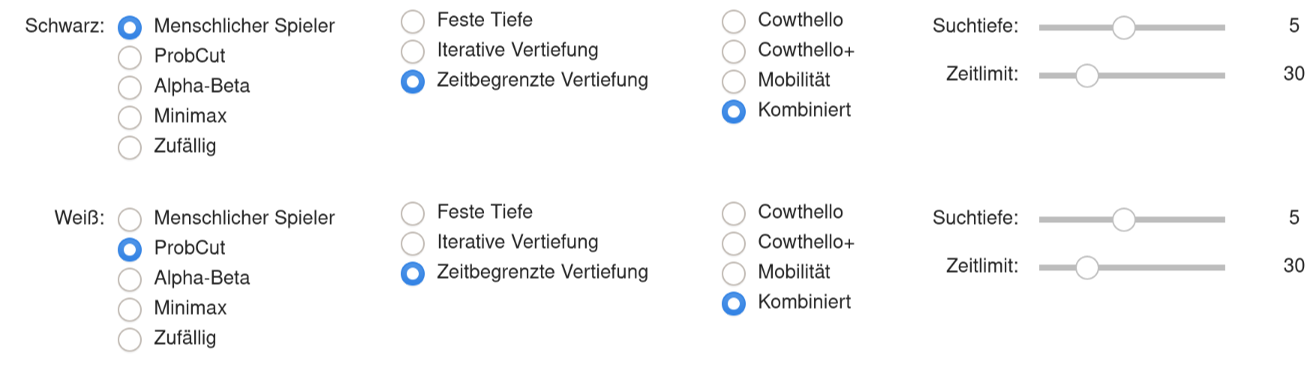
\includegraphics[width=\textwidth]{gui_settings}
    \caption{Grafische Oberfläche zur Konfiguration der Spieler}
    \label{fig:gui_settings}
\end{figure}

Folgender Code dient zum Starten der interaktiven Applikation. Die
Funktion \passthrough{\lstinline!next\_move!} wird für jeden Spielzug
ausgeführt. Ist eine KI an der Reihe, so wird ein Zug der KI
durchgeführt und die Funktion im Anschluss rekursiv für den nächsten Zug
aufgerufen. Ist ein menschlicher Spieler and der Reihe, wird die
Ausführung unterbrochen. Durch einen Klick auf das gewünschte Feld wird
mittels eines Callbacks in der GUI Implementierung der entsprechende Zug
ausgeführt. Im Callback wird auch die Funktion
\passthrough{\lstinline!next\_move!} erneut für den nächsten Zug
aufgerufen. Zu Beginn des Spiels muss die Funktion
\passthrough{\lstinline!next\_move!} einmal aufgerufen werden. Die
Grafische Benutzeroberfläche ist in \autoref{fig:gui_board} zu sehen.

\begin{lstlisting}[language=Python]
state = GameState()
display_board(state)
settings = get_settings()

def next_move(old_state):
    global state
    # Check if/which AI is playing
    ai = settings[state.turn]['algorithm']
    if ai is not None:
        time.sleep(0.2)
        make_move = settings[old_state.turn]['mode']
        depth = settings[state.turn]['depth']
        timelim = settings[state.turn]['timelimit']
        heuristic = settings[old_state.turn]['heuristic']
        intval = timelim if make_move == ai_make_move_id_timelimited else depth
        state = make_move(ai, old_state, intval, heuristic)
        update_output(state)
        if not state.game_over:
            next_move(state)
try:
    next_move(state)
except KeyboardInterrupt:
    pass
\end{lstlisting}

\begin{figure}[H]
    \centering
    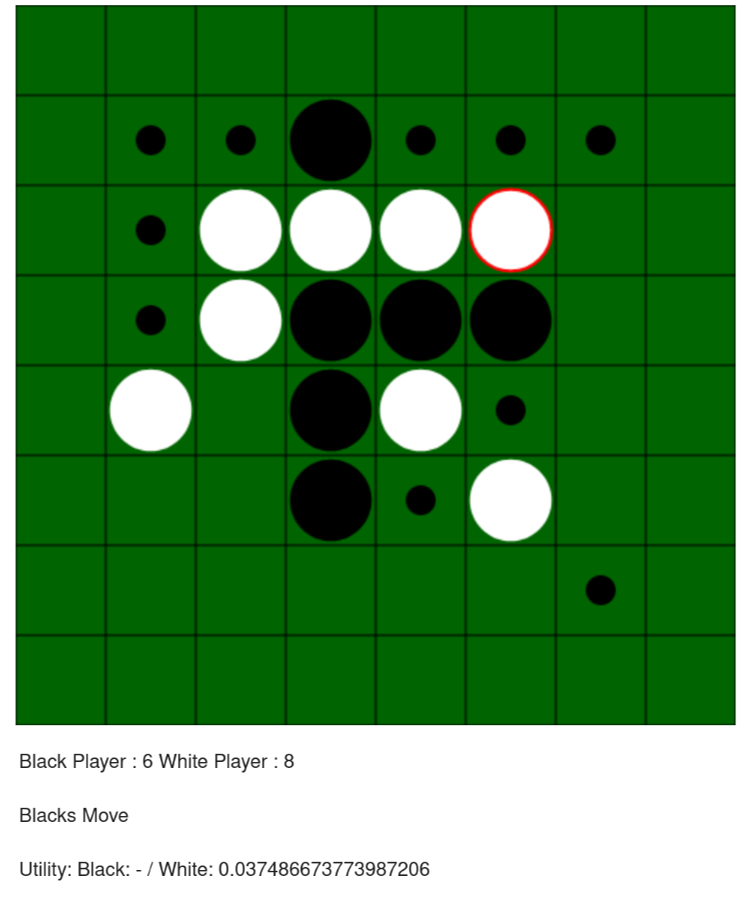
\includegraphics[width=\textwidth]{gui_board}
    \caption{Grafische Oberfläche des Spiels}
    \label{fig:gui_board}
\end{figure}
